\chapter{Introduction}
\section*{Abstract}
Here I give an overview on my thesis.
This includes:
\begin{itemize}
\item general topic
\item field of research: perceptual quality + judgment (relying on memorization and recall?)
\item relevance: why is this question relevant at all? Practical implications?
\item overview on service provider things: acceptance + satisfaction + money stuff
\item my personal motivation to tackle this topic (why important to me?)
\item how am I tackling the question?
\item what can the reader expect? (just hints)
\item (graphic) aspects of multi-episodic QoE: usage duration and time in between + usage pattern + multi-services
\end{itemize}

\section{Goal}
\begin{itemize}
\item How does perceptual quality evolve over multiple interactions (multiple episodes) with the one system/service for one user?
\item How does perceptual overall quality evolve over multiple interactions using a bundle, e.g. more than one system/service for one user? (basically an extension of previous stuff)
\item Goal 1: Find underlying effects temporal effects? (relate them to human memory)
\item Goal 2: Evaluate potential model components for temporal effects (Implement models: either service-independent (better) or service-dependent.)
\end{itemize}
%NOTE: Quality and model must be explained at least minimal here.

\begin{figure}
	\centering
	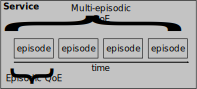
\includegraphics{fig/multi-episodic}
	\caption{Repeated usage episodes with one service and their episodic QoE form a multi-episodic QoE in the user.}
	\label{chap10:img:multiEpisodic}
\end{figure}

\section{Basic definitions}
\begin{itemize}
\item What is \emph{to service}? [Whitepaper] [http://www.merriam-webster.com/dictionary/service] 
\item What is a service, application, system?
\item Telecommunication services + Service Provider %https://www.law.cornell.edu/uscode/text/47/153#50
\end{itemize}

\paragraph*{Service provider's goal}
Make customer happy for as little money as possible for infrastructure: 
\begin{itemize}
\item cost-efficiency: trade-off
\item risk reduction
\item Service usage
\item repeated usage / churn
\end{itemize}

\section{Aspects}
\begin{itemize}
\item QoE as hygienic factor [Moeller, Wechsung]  
\item Money: NPS, Churn, Acceptability, Willingness-to-paying
\item Retainability (sMOS)
\item Adaptive services: service that adjust performance to current conditions (best + economic feasible)
\end{itemize}

\section{Structure}
%TODO Here I describe the structure of my thesis    


A \emph{service provider} provides a \emph{service}\footnote{Please note that the term \emph{service} in this work does not refer to a technical system executed on a server.} that provides a certain "service" to potential users.
In difference to "product creating industries" a service cannot be pre-manufactured, but is rather created on request when needed by a then user., \ie to serve somebody.
%TODO: Performance cannot be determined beforehand! Trust; Service usage lifecycle? Expectations

Before actually deciding to use a service, a potential user must have a need that can be fulfilled by using a service. %proposes to fulfill
If multiple service provider that provide a similar service, a potential user must chose which service to use for fulfillment of his need.
When satisfied with the outcome of using the service a user might interact with the service later on again, whereas a non-satisfying outcome will likely result in not using the same service again and rather use a different one.
In fact, using the same service again, saves time and resource, because the service discovery, evaluation and selection is not conducted.

However, the performance of a service cannot be constant as the service is created on-demand.
The performance of a service might be varying from usage instance to usage instance.
From a user's perspective this might be sufficient, but if the performance some usage instances does meet the expectations / desired performance then a dissatisfaction might occur.
This force the user to abandon the service provider and chose a different one.

This is, in fact, holds for both \emph{physical services} in which a service is provided to user in a physical location often by a person, but also for \emph{telecommunication services}\footnote{Definition as bit pipe as of https://en.wikipedia.org/wiki/Telecommunications_service follow definition of US Communications Act of 1934} like speech telephony or Internet access.
In fact, in telecommunication service are different from classical services as those provide communication between one or more parties, which can be a computer or a person.

In this work, I present my work on the \emph{perceived quality impression} occurring by a human user of telecommunication services.
This work extends prior work by investigating the impact of varying service/system performance on the perceived quality, when the same system(s) are used repeatedly.
This is, in fact, a common case for telecommunication service.
For example a customer of a mobile  provider will use the provided service(s) usually repeatedly, because his telephone number is bound to the service provider and, although it can be transfered to a different provider, this process takes time and effort.
Furthermore, a customer might be bound for a certain extend to a service provider contract duration.
Although contract duration might bind customers to a provider, low performance and thus a low perceived quality affects the future use behavior and increases the churn rate for the end of contract.
In addition, satisfaction and also dissatisfaction of a customers can spread to other customers and potential customers and thus have severe impact on the business performance of a service provider.

In this work I focus on the development of perceived quality over several distinct interactions with a telecommunication service and how a retrospective assessment of the perceived quality of this service is affected by varying service performance.
The actual impact on customer satisfaction and thus business performance of performance variation is not in the scope of this thesis.

The goals of this has two goals:
\paragraph{Goal 1:}


This work is structured as follows: